% Note that the a4paper option is mainly intended so that authors in
% countries using A4 can easily print to A4 and see how their papers will
% look in print - the typesetting of the document will not typically be
% affected with changes in paper size (but the bottom and side margins will).
% Use the testflow package mentioned above to verify correct handling of
% both paper sizes by the user's LaTeX system.
%
% Also note that the "draftcls" or "draftclsnofoot", not "draft", option
% should be used if it is desired that the figures are to be displayed in
% draft mode.
%
\documentclass[conference]{IEEEtran}
%\documentclass[conference,12pt,draftclsnofoot,onecolumn]{IEEEtran}
% Add the compsoc option for Computer Society conferences.
%
% If IEEEtran.cls has not been installed into the LaTeX system files,
% manually specify the path to it like:
% \documentclass[conference]{../sty/IEEEtran}

%\usepackage{lineno}
%\linenumbers



% Some very useful LaTeX packages include:
% (uncomment the ones you want to load)


% *** MISC UTILITY PACKAGES ***
%
%\usepackage{ifpdf}
% Heiko Oberdiek's ifpdf.sty is very useful if you need conditional
% compilation based on whether the output is pdf or dvi.
% usage:
% \ifpdf
%   % pdf code
% \else
%   % dvi code
% \fi
% The latest version of ifpdf.sty can be obtained from:
% http://www.ctan.org/tex-archive/macros/latex/contrib/oberdiek/
% Also, note that IEEEtran.cls V1.7 and later provides a builtin
% \ifCLASSINFOpdf conditional that works the same way.
% When switching from latex to pdflatex and vice-versa, the compiler may
% have to be run twice to clear warning/error messages.






% *** CITATION PACKAGES ***
%
\usepackage{cite}
% cite.sty was written by Donald Arseneau
% V1.6 and later of IEEEtran pre-defines the format of the cite.sty package
% \cite{} output to follow that of IEEE. Loading the cite package will
% result in citation numbers being automatically sorted and properly
% "compressed/ranged". e.g., [1], [9], [2], [7], [5], [6] without using
% cite.sty will become [1], [2], [5]--[7], [9] using cite.sty. cite.sty's
% \cite will automatically add leading space, if needed. Use cite.sty's
% noadjust option (cite.sty V3.8 and later) if you want to turn this off.
% cite.sty is already installed on most LaTeX systems. Be sure and use
% version 4.0 (2003-05-27) and later if using hyperref.sty. cite.sty does
% not currently provide for hyperlinked citations.
% The latest version can be obtained at:
% http://www.ctan.org/tex-archive/macros/latex/contrib/cite/
% The documentation is contained in the cite.sty file itself.






% *** GRAPHICS RELATED PACKAGES ***
%
\ifCLASSINFOpdf
  \usepackage[pdftex]{graphicx}
  % declare the path(s) where your graphic files are
  % \graphicspath{{../pdf/}{../jpeg/}}
  % and their extensions so you won't have to specify these with
  % every instance of \includegraphics
  % \DeclareGraphicsExtensions{.pdf,.jpeg,.png}
\else
  % or other class option (dvipsone, dvipdf, if not using dvips). graphicx
  % will default to the driver specified in the system graphics.cfg if no
  % driver is specified.
  % \usepackage[dvips]{graphicx}
  % declare the path(s) where your graphic files are
  % \graphicspath{{../eps/}}
  % and their extensions so you won't have to specify these with
  % every instance of \includegraphics
  % \DeclareGraphicsExtensions{.eps}
\fi
% graphicx was written by David Carlisle and Sebastian Rahtz. It is
% required if you want graphics, photos, etc. graphicx.sty is already
% installed on most LaTeX systems. The latest version and documentation can
% be obtained at: 
% http://www.ctan.org/tex-archive/macros/latex/required/graphics/
% Another good source of documentation is "Using Imported Graphics in
% LaTeX2e" by Keith Reckdahl which can be found as epslatex.ps or
% epslatex.pdf at: http://www.ctan.org/tex-archive/info/
%
% latex, and pdflatex in dvi mode, support graphics in encapsulated
% postscript (.eps) format. pdflatex in pdf mode supports graphics
% in .pdf, .jpeg, .png and .mps (metapost) formats. Users should ensure
% that all non-photo figures use a vector format (.eps, .pdf, .mps) and
% not a bitmapped formats (.jpeg, .png). IEEE frowns on bitmapped formats
% which can result in "jaggedy"/blurry rendering of lines and letters as
% well as large increases in file sizes.
%
% You can find documentation about the pdfTeX application at:
% http://www.tug.org/applications/pdftex





% *** MATH PACKAGES ***
%
\usepackage[cmex10]{amsmath}
% A popular package from the American Mathematical Society that provides
% many useful and powerful commands for dealing with mathematics. If using
% it, be sure to load this package with the cmex10 option to ensure that
% only type 1 fonts will utilized at all point sizes. Without this option,
% it is possible that some math symbols, particularly those within
% footnotes, will be rendered in bitmap form which will result in a
% document that can not be IEEE Xplore compliant!
%
% Also, note that the amsmath package sets \interdisplaylinepenalty to 10000
% thus preventing page breaks from occurring within multiline equations. Use:
%\interdisplaylinepenalty=2500
% after loading amsmath to restore such page breaks as IEEEtran.cls normally
% does. amsmath.sty is already installed on most LaTeX systems. The latest
% version and documentation can be obtained at:
% http://www.ctan.org/tex-archive/macros/latex/required/amslatex/math/





% *** SPECIALIZED LIST PACKAGES ***
%
%\usepackage{algorithmic}
% algorithmic.sty was written by Peter Williams and Rogerio Brito.
% This package provides an algorithmic environment fo describing algorithms.
% You can use the algorithmic environment in-text or within a figure
% environment to provide for a floating algorithm. Do NOT use the algorithm
% floating environment provided by algorithm.sty (by the same authors) or
% algorithm2e.sty (by Christophe Fiorio) as IEEE does not use dedicated
% algorithm float types and packages that provide these will not provide
% correct IEEE style captions. The latest version and documentation of
% algorithmic.sty can be obtained at:
% http://www.ctan.org/tex-archive/macros/latex/contrib/algorithms/
% There is also a support site at:
% http://algorithms.berlios.de/index.html
% Also of interest may be the (relatively newer and more customizable)
% algorithmicx.sty package by Szasz Janos:
% http://www.ctan.org/tex-archive/macros/latex/contrib/algorithmicx/




% *** ALIGNMENT PACKAGES ***
%
%\usepackage{array}
% Frank Mittelbach's and David Carlisle's array.sty patches and improves
% the standard LaTeX2e array and tabular environments to provide better
% appearance and additional user controls. As the default LaTeX2e table
% generation code is lacking to the point of almost being broken with
% respect to the quality of the end results, all users are strongly
% advised to use an enhanced (at the very least that provided by array.sty)
% set of table tools. array.sty is already installed on most systems. The
% latest version and documentation can be obtained at:
% http://www.ctan.org/tex-archive/macros/latex/required/tools/


%\usepackage{mdwmath}
%\usepackage{mdwtab}
% Also highly recommended is Mark Wooding's extremely powerful MDW tools,
% especially mdwmath.sty and mdwtab.sty which are used to format equations
% and tables, respectively. The MDWtools set is already installed on most
% LaTeX systems. The lastest version and documentation is available at:
% http://www.ctan.org/tex-archive/macros/latex/contrib/mdwtools/


% IEEEtran contains the IEEEeqnarray family of commands that can be used to
% generate multiline equations as well as matrices, tables, etc., of high
% quality.


%\usepackage{eqparbox}
% Also of notable interest is Scott Pakin's eqparbox package for creating
% (automatically sized) equal width boxes - aka "natural width parboxes".
% Available at:
% http://www.ctan.org/tex-archive/macros/latex/contrib/eqparbox/





% *** SUBFIGURE PACKAGES ***
%\usepackage[tight,footnotesize]{subfigure}
% subfigure.sty was written by Steven Douglas Cochran. This package makes it
% easy to put subfigures in your figures. e.g., "Figure 1a and 1b". For IEEE
% work, it is a good idea to load it with the tight package option to reduce
% the amount of white space around the subfigures. subfigure.sty is already
% installed on most LaTeX systems. The latest version and documentation can
% be obtained at:
% http://www.ctan.org/tex-archive/obsolete/macros/latex/contrib/subfigure/
% subfigure.sty has been superceeded by subfig.sty.



%\usepackage[caption=false]{caption}
\usepackage[justification=justified]{caption}
%\usepackage[font=footnotesize]{subfig}
% subfig.sty, also written by Steven Douglas Cochran, is the modern
% replacement for subfigure.sty. However, subfig.sty requires and
% automatically loads Axel Sommerfeldt's caption.sty which will override
% IEEEtran.cls handling of captions and this will result in nonIEEE style
% figure/table captions. To prevent this problem, be sure and preload
% caption.sty with its "caption=false" package option. This is will preserve
% IEEEtran.cls handing of captions. Version 1.3 (2005/06/28) and later 
% (recommended due to many improvements over 1.2) of subfig.sty supports
% the caption=false option directly:
%\usepackage[caption=false,font=footnotesize]{subfig}
%
% The latest version and documentation can be obtained at:
% http://www.ctan.org/tex-archive/macros/latex/contrib/subfig/
% The latest version and documentation of caption.sty can be obtained at:
% http://www.ctan.org/tex-archive/macros/latex/contrib/caption/




% *** FLOAT PACKAGES ***
%
%\usepackage{fixltx2e}
% fixltx2e, the successor to the earlier fix2col.sty, was written by
% Frank Mittelbach and David Carlisle. This package corrects a few problems
% in the LaTeX2e kernel, the most notable of which is that in current
% LaTeX2e releases, the ordering of single and double column floats is not
% guaranteed to be preserved. Thus, an unpatched LaTeX2e can allow a
% single column figure to be placed prior to an earlier double column
% figure. The latest version and documentation can be found at:
% http://www.ctan.org/tex-archive/macros/latex/base/



%\usepackage{stfloats}
% stfloats.sty was written by Sigitas Tolusis. This package gives LaTeX2e
% the ability to do double column floats at the bottom of the page as well
% as the top. (e.g., "\begin{figure*}[!b]" is not normally possible in
% LaTeX2e). It also provides a command:
%\fnbelowfloat
% to enable the placement of footnotes below bottom floats (the standard
% LaTeX2e kernel puts them above bottom floats). This is an invasive package
% which rewrites many portions of the LaTeX2e float routines. It may not work
% with other packages that modify the LaTeX2e float routines. The latest
% version and documentation can be obtained at:
% http://www.ctan.org/tex-archive/macros/latex/contrib/sttools/
% Documentation is contained in the stfloats.sty comments as well as in the
% presfull.pdf file. Do not use the stfloats baselinefloat ability as IEEE
% does not allow \baselineskip to stretch. Authors submitting work to the
% IEEE should note that IEEE rarely uses double column equations and
% that authors should try to avoid such use. Do not be tempted to use the
% cuted.sty or midfloat.sty packages (also by Sigitas Tolusis) as IEEE does
% not format its papers in such ways.





% *** PDF, URL AND HYPERLINK PACKAGES ***
%
%\usepackage{url}
% url.sty was written by Donald Arseneau. It provides better support for
% handling and breaking URLs. url.sty is already installed on most LaTeX
% systems. The latest version can be obtained at:
% http://www.ctan.org/tex-archive/macros/latex/contrib/misc/
% Read the url.sty source comments for usage information. Basically,
% \url{my_url_here}.





% *** Do not adjust lengths that control margins, column widths, etc. ***
% *** Do not use packages that alter fonts (such as pslatex).         ***
% There should be no need to do such things with IEEEtran.cls V1.6 and later.
% (Unless specifically asked to do so by the journal or conference you plan
% to submit to, of course. )


% correct bad hyphenation here
\hyphenation{op-tical net-works semi-conduc-tor}


\begin{document}
%\bibliographystyle{IEEEtran}
%
% paper title
% can use linebreaks \\ within to get better formatting as desired
\title{Image Analysis for Ultra Low Bandwidth Video Surveillance System}


% author names and affiliations
% use a multiple column layout for up to three different
% affiliations
\author{\IEEEauthorblockN{Pratyush Anand, Subrat Kar$^*$}
\IEEEauthorblockA{Dept. of Electrical Engineering,\\
 Indian Institute of Technology Delhi, \\
Hauz Khas, New Delhi \\
email: eey107515@ee.iitd.ac.in, subrat@ee.iitd.ac.in}}

% conference papers do not typically use \thanks and this command
% is locked out in conference mode. If really needed, such as for
% the acknowledgment of grants, issue a \IEEEoverridecommandlockouts
% after \documentclass

% for over three affiliations, or if they all won't fit within the width
% of the page, use this alternative format:
% 
%\author{\IEEEauthorblockN{Michael Shell\IEEEauthorrefmark{1},
%Homer Simpson\IEEEauthorrefmark{2},
%James Kirk\IEEEauthorrefmark{3}, 
%Montgomery Scott\IEEEauthorrefmark{3} and
%Eldon Tyrell\IEEEauthorrefmark{4}}
%\IEEEauthorblockA{\IEEEauthorrefmark{1}School of Electrical and Computer Engineering\\
%Georgia Institute of Technology,
%Atlanta, Georgia 30332--0250\\ Email: see http://www.michaelshell.org/contact.html}
%\IEEEauthorblockA{\IEEEauthorrefmark{2}Twentieth Century Fox, Springfield, USA\\
%Email: homer@thesimpsons.com}
%\IEEEauthorblockA{\IEEEauthorrefmark{3}Starfleet Academy, San Francisco, California 96678-2391\\
%Telephone: (800) 555--1212, Fax: (888) 555--1212}
%\IEEEauthorblockA{\IEEEauthorrefmark{4}Tyrell Inc., 123 Replicant Street, Los Angeles, California 90210--4321}}




% use for special paper notices
%\IEEEspecialpapernotice{(Invited Paper)}




% make the title area
\maketitle


\begin{abstract}
%\boldmath
We propose a solution for efficiently transforming video data over a
delay tolerant network. We extract and transport only relevant features
from the video frame at a minimal computational cost using low cost COTS
embedded environment.
\end{abstract}
% IEEEtran.cls defaults to using nonbold math in the Abstract.
% This preserves the distinction between vectors and scalars. However,
% if the conference you are submitting to favors bold math in the abstract,
% then you can use LaTeX's standard command \boldmath at the very start
% of the abstract to achieve this. Many IEEE journals/conferences frown on
% math in the abstract anyway.

% no keywords




% For peer review papers, you can put extra information on the cover
% page as needed:
% \ifCLASSOPTIONpeerreview
% \begin{center} \bfseries EDICS Category: 3-BBND \end{center}
% \fi
%
% For peerreview papers, this IEEEtran command inserts a page break and
% creates the second title. It will be ignored for other modes.
\IEEEpeerreviewmaketitle



\section{Introduction}
% no \IEEEPARstart
\indent Surveillance systems are ubiquitous and find many applications
in areas such as traffic monitoring, elderly care etc. Therefore, there
is a pressing need to evolve methods for conserving bandwidth while the
video data is transported from the point of acquisition to the point of
observation. Moreover, an increasing number of video sources rely on
resource constrained (bandwidth-limited, delay-tolerant) networks
such as Zigbee, DASH7 specially in smart home applications for the video
transport. With such networks at layer 1 and 2, there is tremendous
need to conserve/preserve the bandwidth needed by each video stream /
all video streams collectively. We propose a method by which a few
pre-processing operations allow us to still carry out the primary
objective - surveillance - while achieving large and impressive savings
on the required bandwidth.\\
\indent Video surveillance system can be integrated with existing home
network, but it is very important to achieve, reduction in amount
of data to be transmitted due to lack of end to end connectivity. A low
data rate node also allows the system to remain in sleep mode for
longer durations and hence prolongs longer battery life.\\
\indent For surveillance data, only a few segments of image need to be
transmitted (the fast changing scenes). Transmitting only significant
features pre-extracted locally from the image can reduce transmission
requirement significantly. However, this minimization of content must
allow reconstruction of the image with relevant details at the other
end. By extracting semantic information from deduced features, we
reduce the data rate even further.\\
\indent Automatic scene analysis, followed by extraction of  desired
information can be complex, specially when application is targeted for
outdoor monitoring. Sometime background of the scene can be fast
changing, while in some other scene ambient light can be different.
Similarly, there can be many other hurdles in the process of automation.
But if an efficient background detection algorithm is chosen then, these
issues can be addressed. Further, the selected algorithm must allow
information extraction almost in real time. With latest research in
computer vision ~\cite{3, 5}, it seems that such a task could be
viable with low cost embedded system.\\
\indent We have to find suitable image analysis algorithms for a
surveillance application which can work with low cost embedded solutions.
We have selected one of best ~\cite{5} background subtraction algorithm.
Skeletonization and information about selected object ontology
has been used as the recognition method. When object is at distance from
the camera then motion features are very helpful in object recognition.
Proposed method has been executed on x86 as well as on ARM11 platform
and the result has been compared. \\
\indent In the  section II we provide a survey of related work done in
recent past. After this, we describe our proposed framework, followed by
the results and conclusions.  At the end, we have also summarized future
work to be done.


\section{Related Work}
% no \IEEEPARstart
The most difficult part of such an implementation is to find an
efficient background estimation algorithm so that moving scene can be
extracted. Features such as Gradient histogram, Gray Scale (HAAR),
color, texture, self-similarity and motion have been used by different
researchers ~\cite{3, 5, 1, 6, 13}. \\
\indent Cucchiara et al. ~\cite{1} and many other have used color
information as the feature for background estimation. But using only
color as a feature might not be sufficient in surveillance applications,
where image resolution is very low. Viola and Jones ~\cite{2} have added
motion along with image intensities, which gives better result in moving
bodies estimation. It works even when foreground image size is low.
Methods based on Gaussian Mixtures Model (GMM) ~\cite{15} have also been
widely used, but they are computationally very expensive.  When
background color is same as foreground color, then texture features
represented by local binary pattern (LBP) ~\cite{3} provides better
result compared to GMM. It is able to extract foreground of a person
standing on moving escalator. Further, features computed at a single
scale can be used to approximate feature at nearby scale. Such
implementations ~\cite{4} accelerate the execution for practical
applications. There is one non-parametric implementation ~\cite{5} known
as Vibe, which decides the background pixel value after comparison with
closest sample selected randomly. In this approach the background model
gets initialized from a single frame itself.\\
\indent Once we have identified the foreground moving part, next
important task is to reduce it's size or extract minimal useful
information out of it. So far, object based video coding such as
~\cite{7}, ~\cite{8} seem to be the best compression techniques.
Commercial algorithms such as MPEG-4 also employ object based coding.
Applications which we have targeted in this work identify the moving
object with minimal computational cost. Shape or skeleton ~\cite{11}
based approach are computationally efficient for such object
recognition. Medial axis transform, distance transform, morphological
and star skeletonization etc ~\cite{9, 10} are different methods
which can be used to find out the skeleton of an object.\\


\section{Proposed Framework}
% no \IEEEPARstart
Our top level application flow can be explained as in Fig. ~\ref{image_pipeline}.
\begin{figure}[!h]
\centering
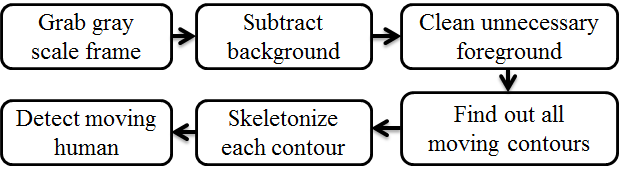
\includegraphics[scale=0.45]{figures/image_pipeline}
\caption{Low BW surveillance image application flow}
\label{image_pipeline}
\end{figure}

\indent Since background subtraction has key role in accomplishing
intended job, therefore we have compared two recently developed
~\cite{3, 5} efficient background subtraction algorithm and then
selected one of them ~\cite{5} in our final work.  The method described
by Yao and Odobez ~\cite{3} is based on use of texture features present
in Local Binary Pattern (LBP).  LBP works well with local illumination
changes, however there can be issues in case of global illumination
change. They have carried out several improvements by using photometric
invariant color measurement and flexible weight updating for background
modes. However, computationally it is not so efficient compared to the
method by Barnich and Van Droogenbroeck ~\cite{5} (Vibe) which we have
used. This algorithm replaces background values for last N frames
randomly.  Furthermore, it diffuses updated values to neighbouring
pixels, and again that too on random basis. So far selected algorithm
surpasses other existing algorithm in computation complexities. Fig.
\ref{bg_compare} shows the comparison of execution times of these two
algorithms.\\
\indent We have used OpenCV library for input and output, i.e.  for
the image frame extraction from a video file or camera and to show the
output result. Vibe object library for background subtraction has been
made available by its author for x86 platform. However, C code has not
been released. Therefore, we have developed our own C code for Vibe so
that we can compile it to be used for ARM platform. Once foreground
frame is extracted, we use OpenCV library function to clean and extract
each moving object.\\

\begin{figure}[!h]
\centering
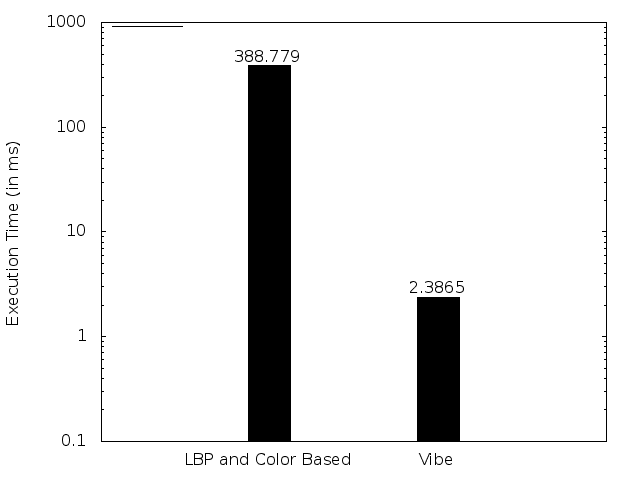
\includegraphics[scale=0.35]{figures/bg_compare}
\caption{Background subtraction average execution time of ~\cite{3} and
~\cite{5}. This timing was observed with a x86 system having DMIPS =
800.}
\label{bg_compare}
\end{figure}

\indent None of the background subtraction algorithms allow complete
foreground extraction. There are always several noise artefacts in the
extracted image. These are removed by morphological operations of
erosion followed by dilation. Further all moving contours are separated
by using standard OpenCV library ~\cite{12} function (cvFindContours)
which gives us boundary points of each moving object.\\

\indent Star skeletonization method has been used to find extreme points
on moving contours. This method plots distance of each boundary point
from the centroid and then uses peaks of the curve as skeleton point.
Next, we identify types of each moving contours using the following
steps.\\
\begin{enumerate}
\item Centroid (C$_x$, C$_y$) of each object is found out.\\
	\begin{equation}
	C_x = {1 \over N} \Sigma ^N _{i = 1} X_i 
	\end{equation}
	\begin{equation}
	C_y = {1 \over N} \Sigma ^N _{i = 1} Y_i 
	\end{equation}
Here X$_i$ and Y$_i$ are (X,Y) co-ordinate of i$_{th}$ point on the contour
boundary. N is total number of points on contour.
\item Distance d$_i$ is calculated between centroid and each boundary
point as follows. This calculated distance vector d$_i$ are stored in an
array.
	\begin{equation}
	d_i = \sqrt{(C_x - X_i)^2 + (C_y - Y_i)^2}, \hspace{10 mm} i =
1,2,3,.....,N
	\end{equation}

\begin{figure}[!h]
\centering
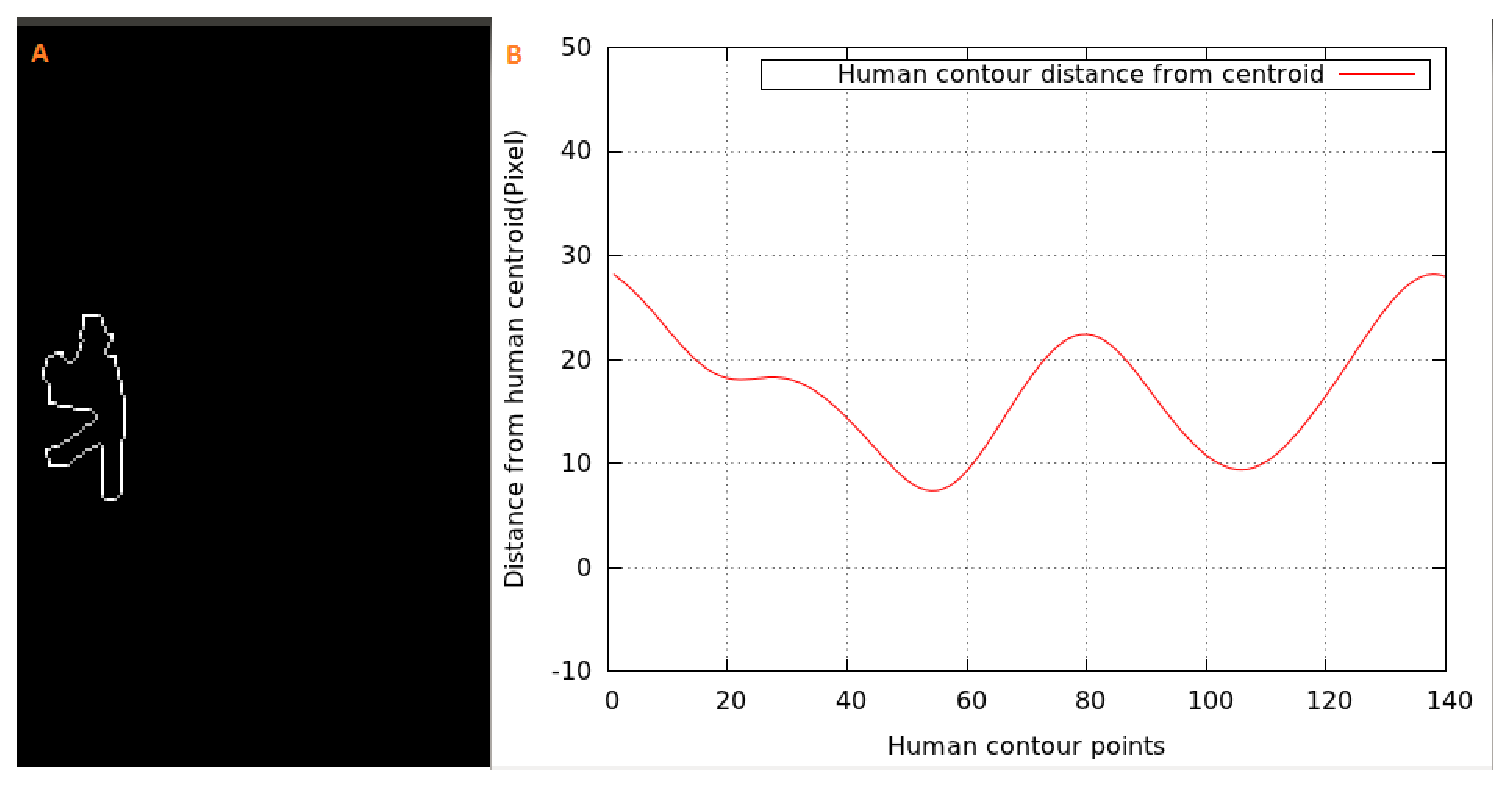
\includegraphics[scale=0.35]{figures/distance}
\caption{(A).Separated human contour. (B). Distance plot of human contour
points from its centroid.}
\label{distance}
\end{figure}

\item The distance vector array is smoothed to remove noise peaks (using
cvSmooth). These distances are plotted  as shown in Fig.
\ref{distance}($B$). Now local maxima of distance vector is calculated
by finding zero crossing of difference vectors.\\
\indent However, even after smoothing operation there are some peaks which is
not of our interest.  In our algorithm, we are using two most relevant
peaks which are nearest to each bottom corner of bounding box of contour
respectively.  Only these two peaks along with centroid will give us
sufficient information to distinguish human from human, vehicle or
animal etc. \\
\indent When the case considered is human, then the two peaks correspond to
the two legs of human. When case considered is vehicle, then the peaks
correspond to the two extrema points of lower portion of back and front.
When it is an animal, then peaks correspond to front and back leg of
animal.\\
\item Let P$_1$(X$_1$, Y$_1$), P$_2$(X$_2$, Y$_2$) and C(C$_x$, C$_y$)
are two peaks nearest to bottom right and bottom left corner and
centroid respectively. Let $\theta$ is the angle between the line
segments P$_1$C and P$_2$C, then $\theta$ can be calculated as
follows.\\
%
	\begin{equation}
	\begin{split}
	\theta = tan^{-1}[(Y_2 - C_y) / (X_2 - C_x)] \\
	 - tan^{-1}[(Y_1 - C_y) / (X_1 - C_x)]
	\end{split}
	\end{equation}
%
\indent If variation of $\theta$ is plotted in respective frames for
human and vehicle then the resultant plot is as shown in Fig.
\ref{angle_plot}.  The observations from this plot is that for a  human
subject, angle variation pattern is repeatable, and it is zero for
almost at regular intervals.  For vehicle, it is constant. The
experiment with images containing animal is yet to be done. For images
with animals in it, there are variations with repeatable patterns but
which never touch zero.  These criterion can be the basis to identify an
object, and to decide whether it is a human,vehicle or animal.

\begin{figure}[!h]
\centering
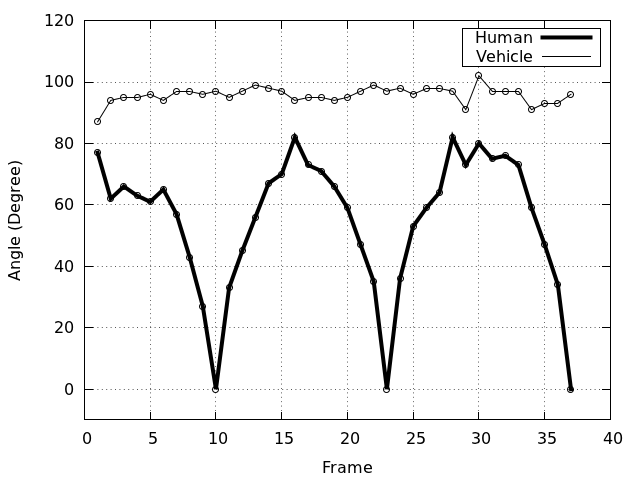
\includegraphics[scale=0.35]{figures/angle_plot}
\caption{Plot of variation of angle $\theta$ with frame number for human and
vehicle.}
\label{angle_plot}
\end{figure}

\item Every new object which comes into the field of view is tracked and
value of (C$_x$, C$_y$), $\theta$ in each frame is stored. 
\begin{enumerate} 
\item We track value of $\theta$ until it goes to zero three times.
\item Now we consider $\theta$ values between first and second zero as
vector T$_1$ and $\theta$ values between second and third zero as vector
T$_2$.
\item We find mean m$_1$ and m$_2$ of vector T$_1$ and T$_2$ respectively.
\item If n is the length of vector T$_1$ then, we calculate correlation
value (r) between these two vectors to find similarities as follows.
	\begin{equation}
	r = {{\Sigma ^n _{i = 1}(T_{1i} - m_1) . (T_{2i} - m_2)}
\over {\sqrt {\Sigma ^n _{i = 1} (T_{1i} - m_1)^2 . \Sigma ^n _{i = 1} (T_{2i}
- m_2)^2}}}
	\end{equation}
\item If correlation value is greater than a threshold value TH$_1$,
then we conclude that it is a human.

\end{enumerate} 
\end{enumerate}
\section{Results}
% no \IEEEPARstart
Since we have used \textbf{S}keleton \textbf{M}otion \textbf{A}nalyzer
for object detection, therefore we name our implementation as SMA.\\
\indent We observe that with SMA, we are able to detect a moving person
after a movement of 3 steps. Fig.  \ref{pipeline_images} shows output
images at different stages of the implementation.\\
\indent We have also done experiments with negative images like a person
moving on bicycle, or a vehicle moving on road. SMA is successfully able
to discriminate between these objects. Fig. \ref{negative_inputs} shows
how it rejects moving vehicle and bicycle and  does not detect them as
human.\\
\begin{figure}[!h]
\centering
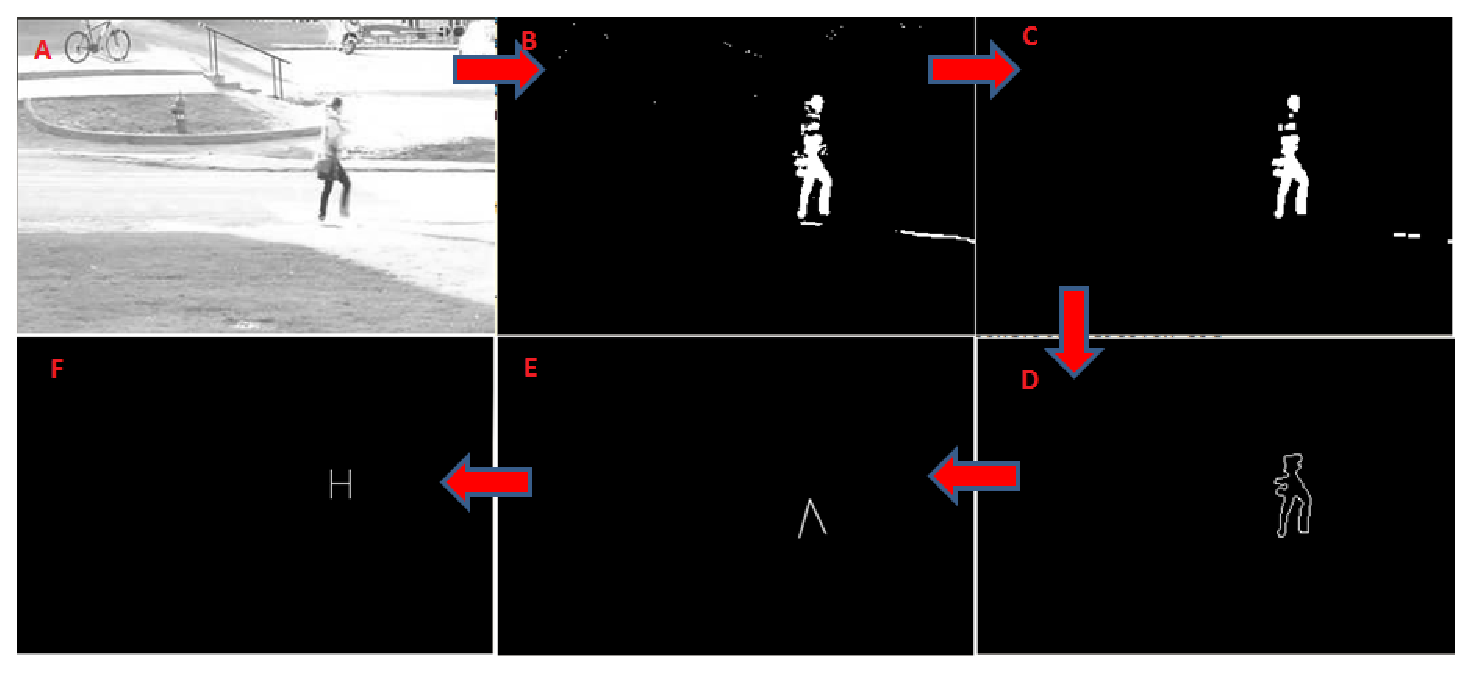
\includegraphics[scale=0.30]{figures/pipeline_images}
\caption{Images at different stages of processing. (From top left in
clockwise order) \textbf{(a.)} Gray Scale input frame 
\textbf({b.)}Foreground extracted image using Vibe \textbf{(c.)} Cleaned
image \textbf{(d.)} Contour of moving object \textbf{(e.)} Plot of three points
of interest, centroid and two distance peaks nearer to bottom left and
bottom right corner of bounding box \textbf{(f.)} Virtual representation
of scene} 
\label{pipeline_images}
\end{figure}

\begin{figure}[!h]
\centering
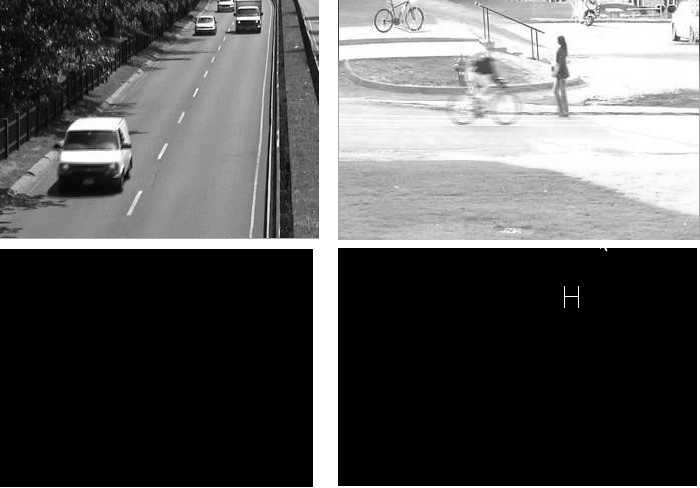
\includegraphics[scale=0.30]{figures/negative_inputs}
\caption{Input and output images in case of negative images}
\label{negative_inputs}
\end{figure}

\indent We have implemented and executed SMA, HAAR ~\cite{2} and
covariance ~\cite{19} feature based detection algorithm at both x86
desktop computer and embedded ARM platform. Comparison of execution time
has been shown in Fig.  \ref{pipeline_execution_time}. It shows a
definite improvement in execution speed of SMA over HAAR and covariance
feature based approach.  SMA takes just 3.6 ms on the average, while
HAAR and covariance feature based algorithm take around 20 ms and 248 ms
respectively per frame at x86 platform having DMIPS = 800. Comparison of
timing at ARM platform with DMIPS = 44 shows that SMA takes 182 ms
on the average, while HAAR and covariance feature based algorithm take
around 942 ms and 4.65 s respectively per frame.  \\
\begin{figure}[!h]
\centering
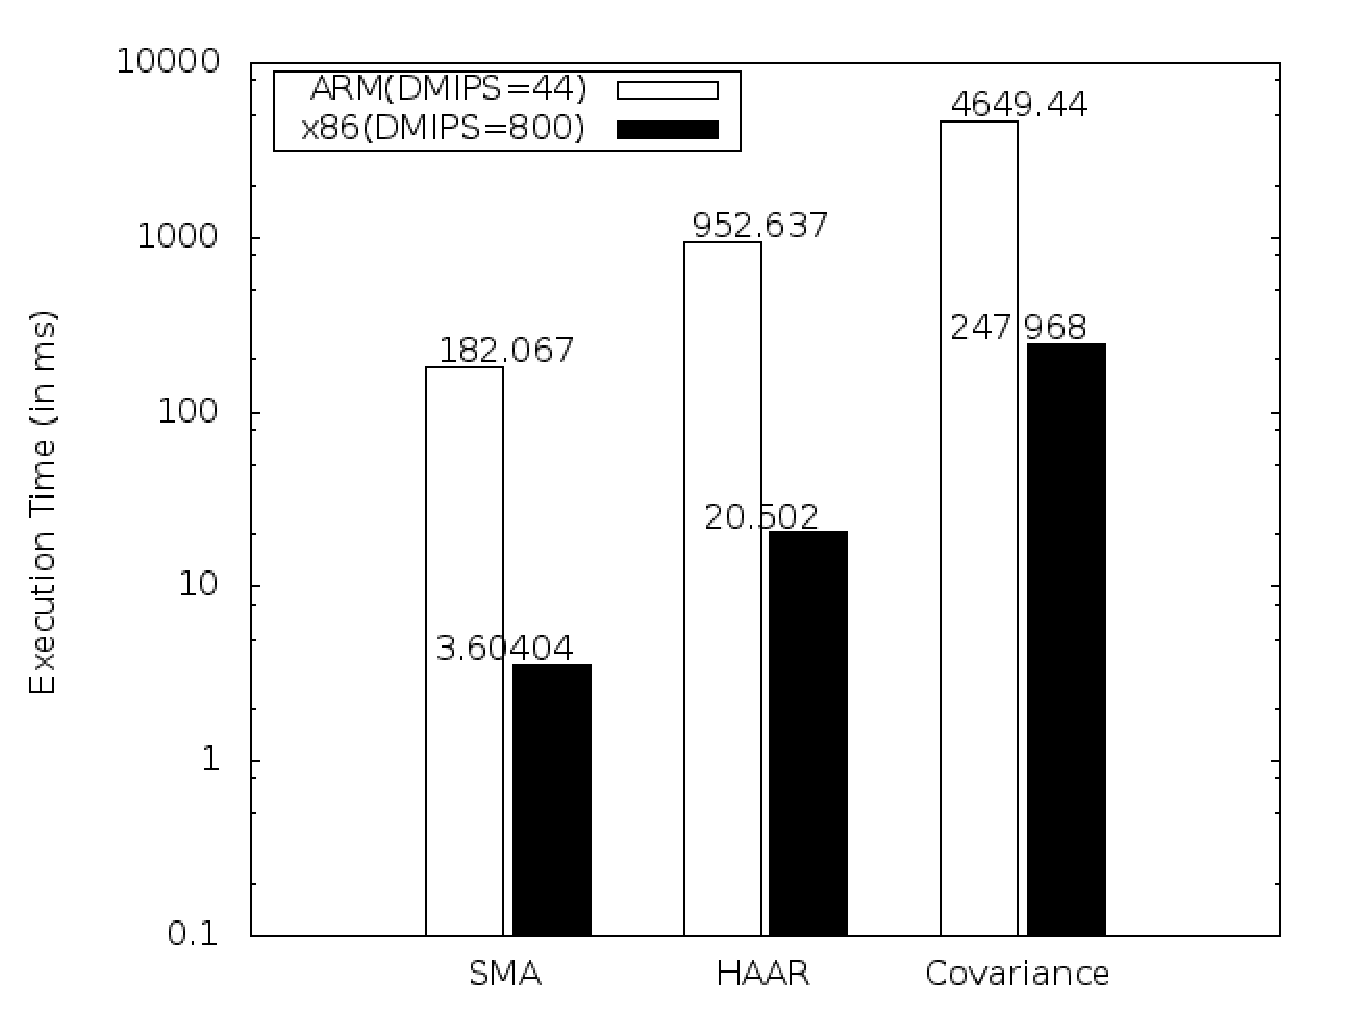
\includegraphics[scale=0.30]{figures/pipeline_execution_time}
\caption{Execution time of evaluated algorithms at ARM and x86
platform}
\label{pipeline_execution_time}
\end{figure}

Therefore, if a surveillance application requires to identify moving person,
then we might not need to use complex algorithm to get real time
performance with low cost embedded platform. By using the proposed
algorithm, we need far less computational power.

\section{Future Work}
% no \IEEEPARstart

We need to see that how does this implementation behaves with existing home
networks like zigbee. Vibe algorithm has one issue that it is not able to
remove shadow. So, an improvement in Vibe for ghost and shadow removal
will make it more robust.


% An example of a floating figure using the graphicx package.
% An example of a floating figure using the graphicx package.
% Note that \label must occur AFTER (or within) \caption.
% For figures, \caption should occur after the \includegraphics.
% Note that IEEEtran v1.7 and later has special internal code that
% is designed to preserve the operation of \label within \caption
% even when the captionsoff option is in effect. However, because
% of issues like this, it may be the safest practice to put all your
% \label just after \caption rather than within \caption{}.
%
% Reminder: the "draftcls" or "draftclsnofoot", not "draft", class
% option should be used if it is desired that the figures are to be
% displayed while in draft mode.
%
%\begin{figure}[!t]
%\centering
%\includegraphics[width=2.5in]{myfigure}
% where an .eps filename suffix will be assumed under latex, 
% and a .pdf suffix will be assumed for pdflatex; or what has been declared
% via \DeclareGraphicsExtensions.
%\caption{Simulation Results}
%\label{fig_sim}
%\end{figure}

% Note that IEEE typically puts floats only at the top, even when this
% results in a large percentage of a column being occupied by floats.


% An example of a double column floating figure using two subfigures.
% (The subfig.sty package must be loaded for this to work.)
% The subfigure \label commands are set within each subfloat command, the
% \label for the overall figure must come after \caption.
% \hfil must be used as a separator to get equal spacing.
% The subfigure.sty package works much the same way, except \subfigure is
% used instead of \subfloat.
%
%\begin{figure*}[!t]
%\centerline{\subfloat[Case I]\includegraphics[width=2.5in]{subfigcase1}%
%\label{fig_first_case}}
%\hfil
%\subfloat[Case II]{\includegraphics[width=2.5in]{subfigcase2}%
%\label{fig_second_case}}}
%\caption{Simulation results}
%\label{fig_sim}
%\end{figure*}
%
% Note that often IEEE papers with subfigures do not employ subfigure
% captions (using the optional argument to \subfloat), but instead will
% reference/describe all of them (a), (b), etc., within the main caption.


% An example of a floating table. Note that, for IEEE style tables, the 
% \caption command should come BEFORE the table. Table text will default to
% \footnotesize as IEEE normally uses this smaller font for tables.
% The \label must come after \caption as always.
%
%\begin{table}[!t]
%% increase table row spacing, adjust to taste
%\renewcommand{\arraystretch}{1.3}
% if using array.sty, it might be a good idea to tweak the value of
% \extrarowheight as needed to properly center the text within the cells
%\caption{An Example of a Table}
%\label{table_example}
%\centering
%% Some packages, such as MDW tools, offer better commands for making tables
%% than the plain LaTeX2e tabular which is used here.
%\begin{tabular}{|c||c|}
%\hline
%One & Two\\
%\hline
%Three & Four\\
%\hline
%\end{tabular}
%\end{table}


% Note that IEEE does not put floats in the very first column - or typically
% anywhere on the first page for that matter. Also, in-text middle ("here")
% positioning is not used. Most IEEE journals/conferences use top floats
% exclusively. Note that, LaTeX2e, unlike IEEE journals/conferences, places
% footnotes above bottom floats. This can be corrected via the \fnbelowfloat
% command of the stfloats package.



\section{Conclusion}

\indent We have exploited the unique property of human leg motion, that
it is periodic and also angle between two legs varies between zero and a
maximum value.  We have demonstrated that with our proposed framework
one can achieve almost real time pedestrian detection even with low cost
embedded platforms, making it viable for implementation for low cost
vision/surveillance platform.



% conference papers do not normally have an appendix


% use section* for acknowledgement
%\section*{Acknowledgment}




% trigger a \newpage just before the given reference
% number - used to balance the columns on the last page
% adjust value as needed - may need to be readjusted if
% the document is modified later
%\IEEEtriggeratref{8}
% The "triggered" command can be changed if desired:
%\IEEEtriggercmd{\enlargethispage{-5in}}

% references section

% can use a bibliography generated by BibTeX as a .bbl file
% BibTeX documentation can be easily obtained at:
% http://www.ctan.org/tex-archive/biblio/bibtex/contrib/doc/
% The IEEEtran BibTeX style support page is at:
% http://www.michaelshell.org/tex/ieeetran/bibtex/
\bibliographystyle{IEEEtran}
% argument is your BibTeX string definitions and bibliography database(s)
%\bibliography{IEEEabrv,../bib/paper}
%
% <OR> manually copy in the resultant .bbl file
% set second argument of \begin to the number of references
% (used to reserve space for the reference number labels box)
%\begin{thebibliography}{1}

%\bibitem{1}
%H.~Kopka and P.~W. Daly, \emph{A Guide to \LaTeX}, 3rd~ed.\hskip 1em plus
%  0.5em minus 0.4em\relax Harlow, England: Addison-Wesley, 1999.

%\end{thebibliography}

\bibliography{references}


% that's all folks
\end{document}


